
\section{OPIL Data Model}\label{sec:model}

The section describes the OPIL data model in detail.  
OPIL classes are in general organized in pairs, one for specifying the interface to a protocol, the other for making requests to execute protocol via that interface.
As such, this section is also organized in pairs, first each interface class, then the complementary request class.

\todo[inline]{Change PI SampleSet to a new FactorSpace class?}

\subsection{ProtocolInterface}
\label{sec:ProtocolInterface}

The \opil{ProtocolInterface} class represents a protocol that is make available for use in requests for experiments.

\begin{figure}[ht]
\begin{center}
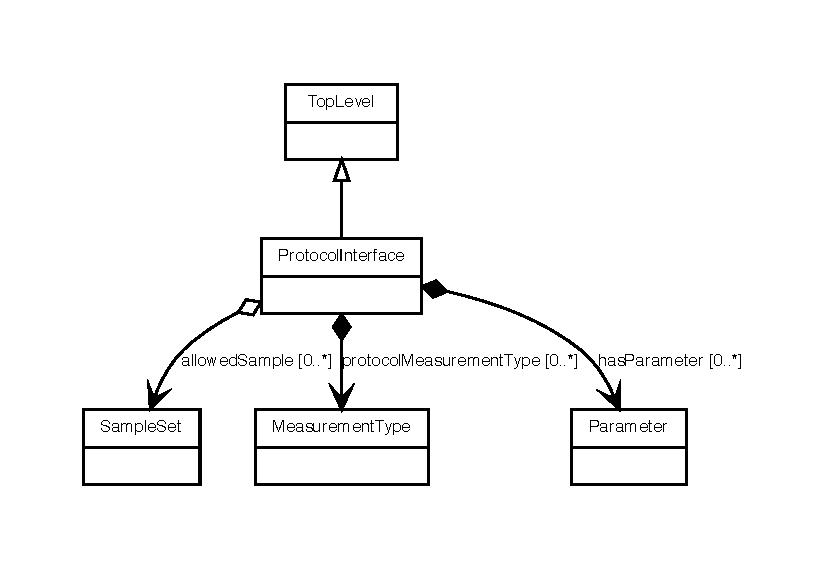
\includegraphics[scale=0.8]{figures/ProtocolInterface}
\caption[]{Diagram of the \opil{ProtocolInterface} class and its associated properties}
\label{uml:ProtocolInterface}
\end{center}
\end{figure}

\begin{itemize}
\item \label{sec:hasSampleSet}
The \opil{hasSampleSet} property MAY contain any number of \opil{URI}s, each of which refers to a \opil{SampleSet} object that describes a range of sample designs allowed for this protocol.
Any sample design whose properties fall into the range defined for any such \opil{SampleSet} SHOULD be accepted for execution of the protocol.
For example, a sample set might indicate that a protocol is intended for use with any strain of {\it E. coli} in any growth media with a concentration of one small-molecule inducer at a concentration between 0 and 1 $\mu$M.

\item \label{sec:hasParameter}
The \opil{hasParameter} property MAY contain any number of \opil{URI}s, each of which refers to a \opil{Parameter} object that describes one of the global parameters used to control the behavior of the protocol. 
For example, a \opil{Parameter} might be used for indicating the range of temperatures that can be requested for a culturing stage or the range of speeds for centrifuging.

\item \label{sec:hasMeasurementType}
The \opil{hasMeasurementType} property MAY contain any number of \opil{URI}s, each of which refers to a \opil{MeasurementType} object that describes a type of instrument that can be used to produce data from this protocol.
For example, a \opil{MeasurementType} might indicate that the protocol can read absorbance from a plate reader up to once every 10 minutes.
\end{itemize}

\subsection{ExperimentalRequest}
\label{sec:ExperimentalRequest}

The \opil{ExperimentalRequest} class is used to describe requests to actually run a particular protocol.

\begin{figure}[ht]
\begin{center}
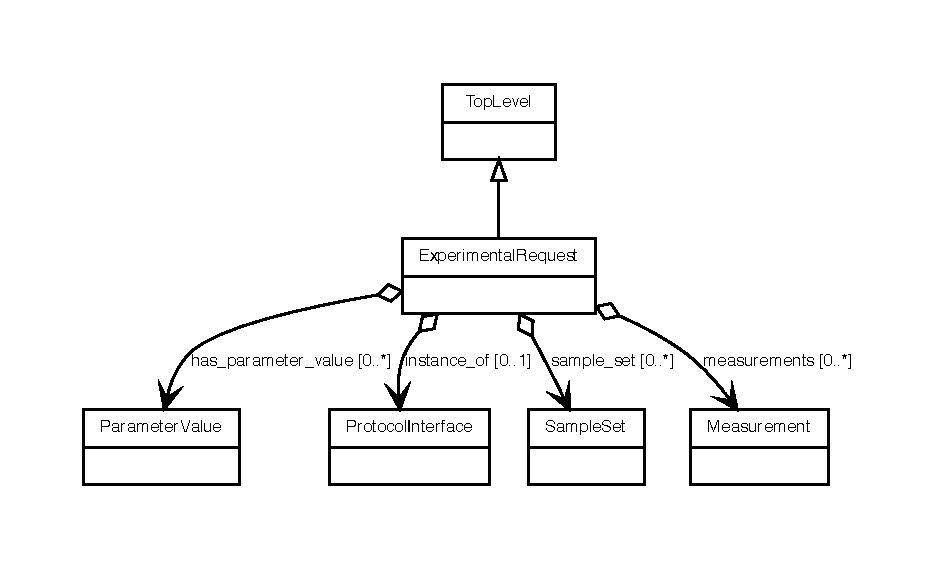
\includegraphics[scale=0.8]{figures/ExperimentalRequest}
\caption[]{Diagram of the \opil{ExperimentalRequest} class and its associated properties}
\label{uml:ExperimentRequest}
\end{center}
\end{figure}

\begin{itemize}
\item \label{sec:ER:instanceOf}
The \opilmult{ER:instanceOf}{instanceOf} property is REQUIRED and MUST contain a single \opil{URI} that refers to the \opil{ProtocolInterface} describing the protocol to be run.

\item \label{sec:hasSampleSet}
The \opil{hasSampleSet} property MAY contain any number of \opil{URI}s, each of which refers to a \opil{SampleSet} object that describes a collection of samples to be run through the experiment.
The total collection of samples requested is the union of all referred \opil{SampleSet} objects.

For example, a sample set might indicate that a protocol is intended for run in triplicate for a positive control strain, negative control strain, and four experimental strains, each at five different levels of inducer and in three different types of media (270 samples), and a second separate sample set might be used to request two replicates each of media-only control for each of the three media (6 samples), for a total of 276 samples.

\item \label{sec:hasMeasurement}
The \opil{hasMeasurement} property MAY contain any number of \opil{URI}s, each of which refers to a \opil{Measurement} object that sets the measurements to be collected during the execution of the protocol.
The total collection of measurements requested is the union of all referred \opil{SampleSet} objects.

For example, a \opil{Measurement} might be used to request plate reader absorbance data be collected at hours 0, 6, and 12, and a second \opil{Measurement} might be used to request that flow cytometry data be collected at hour 12.

\item \label{sec:hasParameterValue}
The \opil{hasParameterValue} property MAY contain any number of \opil{URI}s, each of which refers to a \opil{ParameterValue} object that sets one of the global parameters used to control the behavior of the protocol. 
To prevent conflicts between values, any two \opil{ParameterValue} object thus referred to MUST NOT be a \opil{valueOf} same \opil{Parameter} (e.g., culturing temperature cannot simultaneously be both 30 and  37 degrees Celsius).

For example, a \opil{ParameterValue} might be used to request that culturing temperature be set to 37 degrees Celsius and another used to set centrifuging to 5000 rpm.

\end{itemize}



\subsection{SampleSet}
\label{sec:SampleSet}

The \opil{SampleSet} class is an extension of \sbol{CombinatorialDerivation}, which adds the information of how many replicates should be executed for each specified sample in the combinatorial collection.

\begin{figure}[ht]
\begin{center}
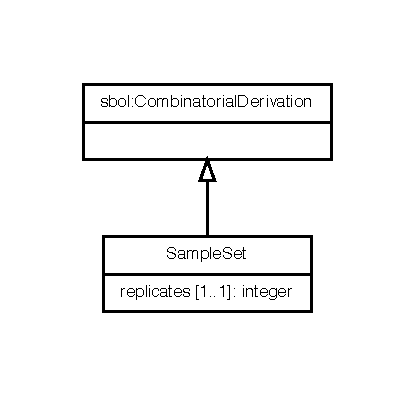
\includegraphics[scale=0.8]{figures/SampleSet}
\caption[]{Diagram of the \opil{SampleSet} class and its associated properties}
\label{uml:SampleSet}
\end{center}
\end{figure}

\begin{itemize}
\item \label{sec:replicates}
The \opil{replicates} property is REQUIRED and MUST contain a single positive \opil{integer} that indicates the number of replicates of each sample that should be run.
\end{itemize}


\subsection{MeasurementType}
\label{sec:MeasurementType}

The \opil{MeasurementType} class is used to indicate when and how often a particular modality of measurement is allowed to be used.
For example, it might be used to say that plate reader data is required to be taken, and that it can be taken up to three times in the range of 12 to 24 hours, no more frequently than once per hour.

\begin{figure}[ht]
\begin{center}
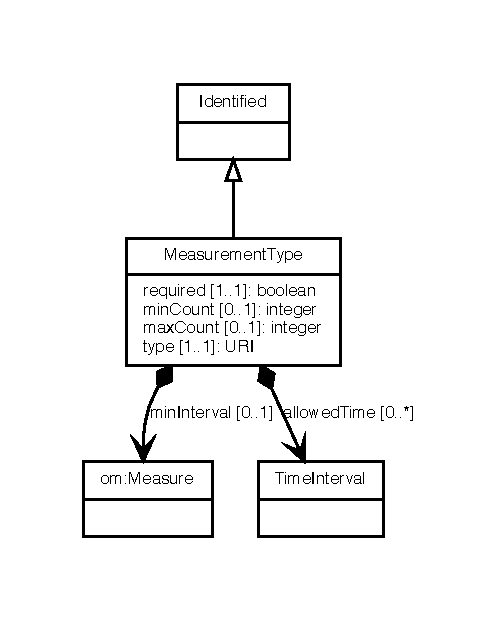
\includegraphics[scale=0.8]{figures/MeasurementType}
\caption[]{Diagram of the \opil{MeasurementType} class and its associated properties}
\label{uml:MeasurementType}
\end{center}
\end{figure}

\todo[inline]{Should we delete the required field, as redundant with minCount?}

\begin{itemize}
\item \label{sec:type}
The \opil{type} property is REQUIRED and MUST contain a \opil{URI} indicating the nature of the measurement being indicated.
When possible, this value SHOULD be drawn from the NCIT ontology's Instrumentation (\url{https://identifiers.org/NCIT:C16742}) or Laboratory Procedure (\url{https://identifiers.org/C25294}) branch.
A list of RECOMMENDED terms for common assays is provided in \ref{tbl:measurement_types}.

\item \label{sec:required}
The \opil{required} property is REQUIRED and MUST contain a \opil{boolean} indicating whether this type of measurement must be used during the execution of the protocol. 
For example, a protocol might always produce plate reader measurements (\opil{required} is true), but have proteomics optional (\opil{required} is false).

\item \label{sec:minCount}
The \opil{minCount} property is OPTIONAL and MAY contain a non-negative \opil{integer} indicating that this \\\opil{MeasurementType} MUST be requested at least the indicated number of times.
If \opil{minCount} is not set, it is treated as zero (or one if \opil{required} is true).
\opil{minCount} must be less than or equal to \opil{maxCount}.

\item \label{sec:maxCount}
The \opil{maxCount} property is OPTIONAL and MAY contain a non-negative \opil{integer} indicating that this \\\opil{MeasurementType} MUST NOT be requested more than the indicated number of times.
If \opil{maxCount} is not set, it is treated as infinity.
\opil{maxCount} must be greater than or equal to \opil{minCount}.


\item \label{sec:minInterval}
The \opil{minInterval} property is OPTIONAL and MAY contain a \opil{URI} referring to a \om{Measure} with a time duration unit indicating the minimum time between two subsequent measurements taken with this modality.
For example, setting \opil{minInterval} to a \om{Measure} specifying one hour would indicate that no two times when this \opil{MeasurementType} is requested may be less than one hour apart.
If \opil{minInterval} is not set, it is treated as zero.

\item \label{sec:allowedTime}
The \opil{allowedTime} property MAY contain any number of \opil{URI}s, each referring to a \opil{TimeInterval} that specifies a range of valid times.
The total set of valid times is the union of all such \opil{TimeInterval}s.
For example, one \opil{TimeInterval} could be used to indicate that the plate reader can be used right at the beginning of the protocol (time 0 hours), then again during the interval of 12 to 24 hours after it began.
If \opil{allowedTime} is not set, then all times are allowed.
\end{itemize}

\begin{table}[ht]
  \begin{edtable}{tabular}{ll}
    \toprule
    \textbf{Measurement Type} & \textbf{URI for NCIT Term} \\
    \midrule
    Flow cytometer & \url{https://identifiers.org/NCIT:C78806}\\
    Microplate reader & \url{https://identifiers.org/NCIT:C70661}\\
    RNAseq & \url{https://identifiers.org/NCIT:C124261}\\
    Fluorescence Microscopy & \url{https://identifiers.org/NCIT:C16856}\\
    \bottomrule
  \end{edtable}
  \caption{Partial list of NCIT terms to specify common assays using the \opil{type} property of a \opil{MeasurementType}}.
 \label{tbl:measurement_types}
\end{table}


\subsubsection{TimeInterval}
\label{sec:TimeInterval}

\todo[inline]{Fold in with factor space, if we do that?}

\opil{TimeInterval} is used for specifying valid ranges of time in which a measurement is allowed to be taken.
For example, it might be used to say that a measurement can be taken anywhere in the range of 12 to 24 hours, or might be used to say that measurements cannot be taken before hour 3.

\begin{figure}[ht]
\begin{center}
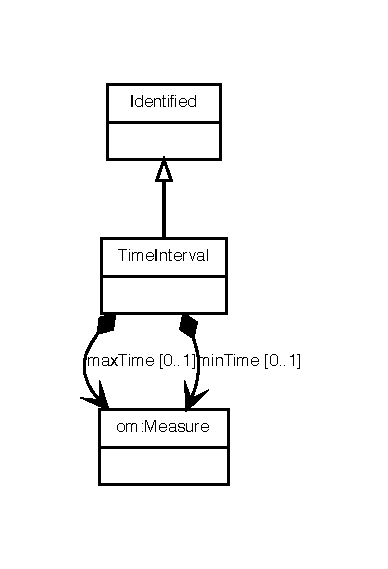
\includegraphics[scale=0.8]{figures/TimeInterval}
\caption[]{Diagram of the \opil{TimeInterval} class and its associated properties}
\label{uml:TimeInterval}
\end{center}
\end{figure}

\begin{itemize}
\item \label{sec:minTime}
The \opil{minTime} property is OPTIONAL and MAY contain a \opil{URI} referring to a \om{Measure} with a time duration unit.
If \opil{minTime} is not set, it is treated as zero.
\opil{minTime} must be less than or equal to \opil{maxTime}.

\item \label{sec:maxTime}
The \opil{maxTime} property is OPTIONAL and MAY contain a \opil{URI} referring to a \om{Measure} with a time duration unit.
If \opil{maxTime} is not set, it is treated as infinity.
\opil{maxTime} must be greater than or equal to \opil{minTime}.
\end{itemize}


\subsection{Measurement}
\label{sec:Measurement}

The \opil{Measurement} class is used to request that a particular measurement be performed at certain times.
For example, it might be used to request that a plate reader be used at hours 0, 6, and 12.

\begin{figure}[ht]
\begin{center}
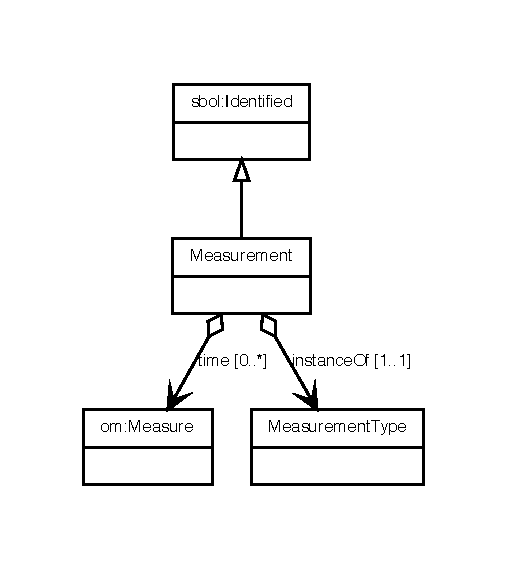
\includegraphics[scale=0.8]{figures/Measurement}
\caption[]{Diagram of the \opil{Measurement} abstract class and its associated properties}
\label{uml:Measurement}
\end{center}
\end{figure}

\begin{itemize}
\item \label{sec:M:instanceOf}
The \opilmult{M:instanceOf}{instanceOf} property is REQUIRED and MUST contain a single \opil{URI} that refers to the \opil{MeasurementType} describing the measurement to be taken.

\item \label{sec:time}
The \opil{time} property MAY contain any number of \opil{URI}s, each referring to a \om{Measure} with a time unit.
\end{itemize}





\subsection{Parameter}
\label{sec:Parameter}

\todo[inline]{Should type be transformed from class type to a field on Parameter, except for the ones that actually have additional fields? This would simplify type-matching validation rules, but add complexity to knowing when an extension is necessary. The EnumeratedParameter allowedValue field could certainly generalize to any. Likewise, the min and max could be generalized for any orderable type (and maybe folded in with factor spaces, if we do that).}
\todo[inline]{I think we need an additional field here to indicate whether a parameter is required or not}

\opil{Parameter} is an abstract class that represents any sort of global setting that may be provided to configure the execution of a protocol.
The subclasses of \opil{Parameter} are used to indicate different types of value to be set, such as Booleans, integers, and measures (i.e., floating point values with units).

This is a catch-all class intended for capturing any information that cannot be systematized in terms of \opil{SampleSet} and \opil{Measurement} information, and thus SHOULD NOT be used to represent anything that can be well-represented using those classes.

For example, a \opil{Parameter} can be used to determine whether an optional post-culturing dilution step should be executed.
A \opil{Parameter} SHOULD NOT be used to determine which culture media should be used in a sample (since that can be represented well via \opil{SampleSet}) or to indicate whether samples should be evaluated with an optional proteomics step (since that can be represented well via \opil{Measurement}).



\begin{figure}[ht]
\begin{center}
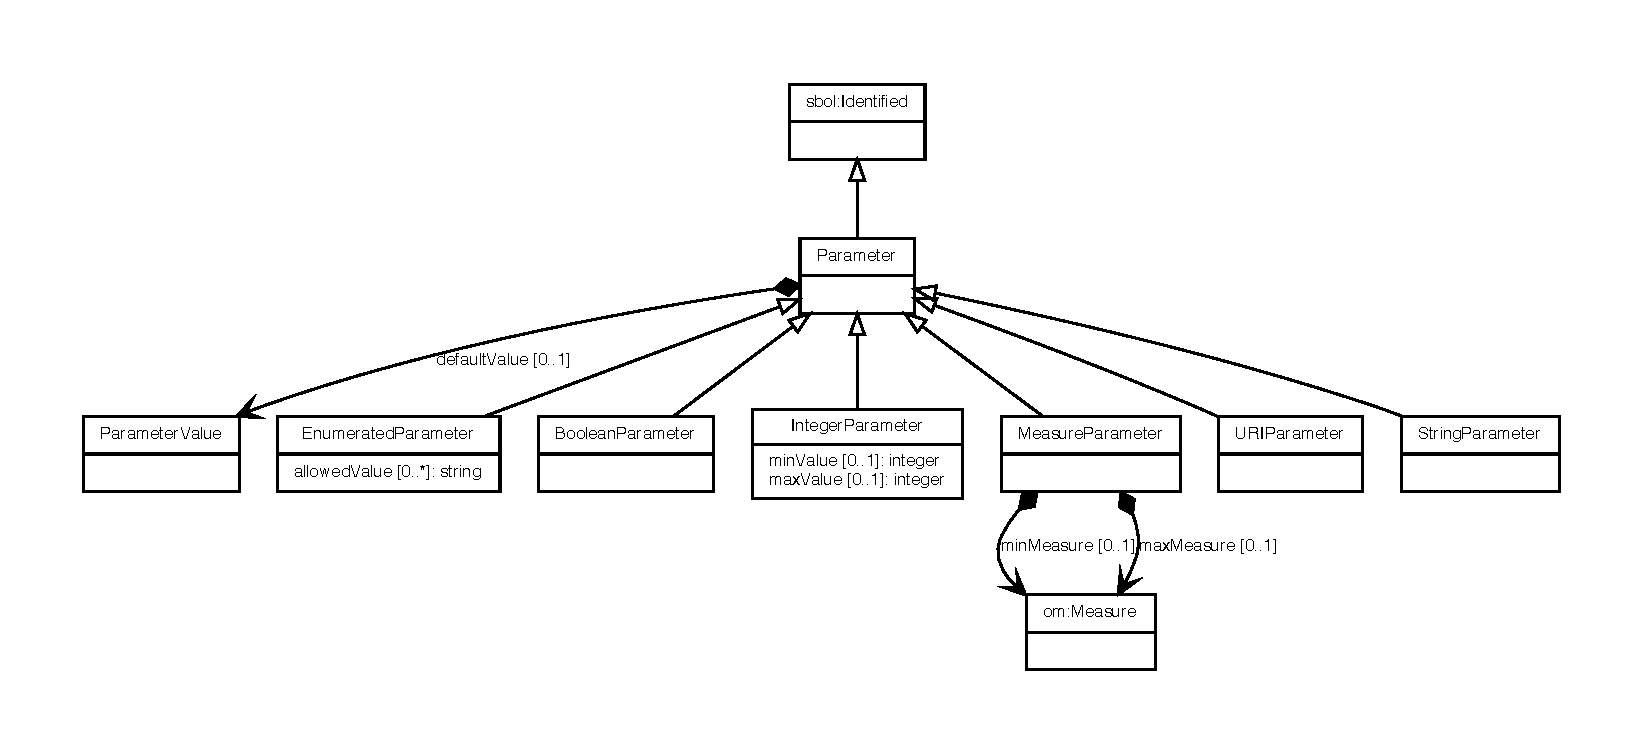
\includegraphics[scale=0.6]{figures/Parameter_definition_and_abstraction}
\caption[]{Diagram of the \opil{Parameter} abstract class and its associated properties and subclasses}
\label{uml:Parameter}
\end{center}
\end{figure}

\begin{itemize}
\item \label{sec:defaultValue}
The \opil{defaultValue} property is OPTIONAL and MAY contain a single \opil{URI} that refers to a \opil{ParameterValue} that provides a default value for the parameter in the case that it is not set.
\end{itemize}


\subsubsection{BooleanParameter}
\label{sec:BooleanParameter}

{\em \opil{BooleanParameter} has no additional properties.}

\subsubsection{EnumeratedParameter}
\label{sec:EnumeratedParameter}

\begin{itemize}
\item \label{sec:allowedValue}
The \opil{allowedValue} property MAY contain any number of \opil{string} values, indicating the legal values for this \opil{EnumeratedParameter}. 
For example, 
\end{itemize}

\subsubsection{IntegerParameter}
\label{sec:IntegerParameter}

\begin{itemize}
\item \label{sec:minValue}
The \opil{minValue} property is OPTIONAL and MAY contain an \opil{integer}.
If \opil{minValue} is not set, it is treated as negative infinity.
\opil{minValue} must be less than or equal to \opil{maxValue}.

\item \label{sec:maxValue}
The \opil{maxValue} property is OPTIONAL and MAY contain an \opil{integer}.
If \opil{maxValue} is not set, it is treated as infinity.
\opil{maxValue} must be greater than or equal to \opil{minValue}.
\end{itemize}

\subsubsection{MeasureParameter}
\label{sec:MeasureParameter}

\begin{itemize}
\item \label{sec:minMeasure}
The \opil{minMeasure} property is OPTIONAL and MAY contain a \opil{URI} referring to a \om{Measure}.
If \opil{minMeasure} is not set, it is treated as negative infinity.
\opil{minMeasure} must be less than or equal to \opil{maxMeasure}.

\item \label{sec:maxMeasure}
The \opil{maxMeasure} property is OPTIONAL and MAY contain a \opil{URI} referring to a \om{Measure}.
If \opil{maxMeasure} is not set, it is treated as infinity.
\opil{maxMeasure} must be greater than or equal to \opil{minMeasure}.
\end{itemize}

\subsubsection{StringParameter}
\label{sec:StringParameter}

{\em \opil{BooleanParameter} has no additional properties.}

\subsubsection{URIParameter}
\label{sec:URIParameter}

{\em \opil{BooleanParameter} has no additional properties.}


\subsection{ParameterValue}
\label{sec:ParameterValue}

\opil{ParameterValue} is an abstract class is used to set a parameter for a protocol to a particular value. 
The subclasses of \opil{ParameterValue} are used for different types of value to be set, such as Booleans, integers, and measures (i.e., floating point values with units).
For example, a \opil{MeasureValue} might be used to request that a centrifuging step be run at 5000 rpm.

\begin{figure}[ht]
\begin{center}
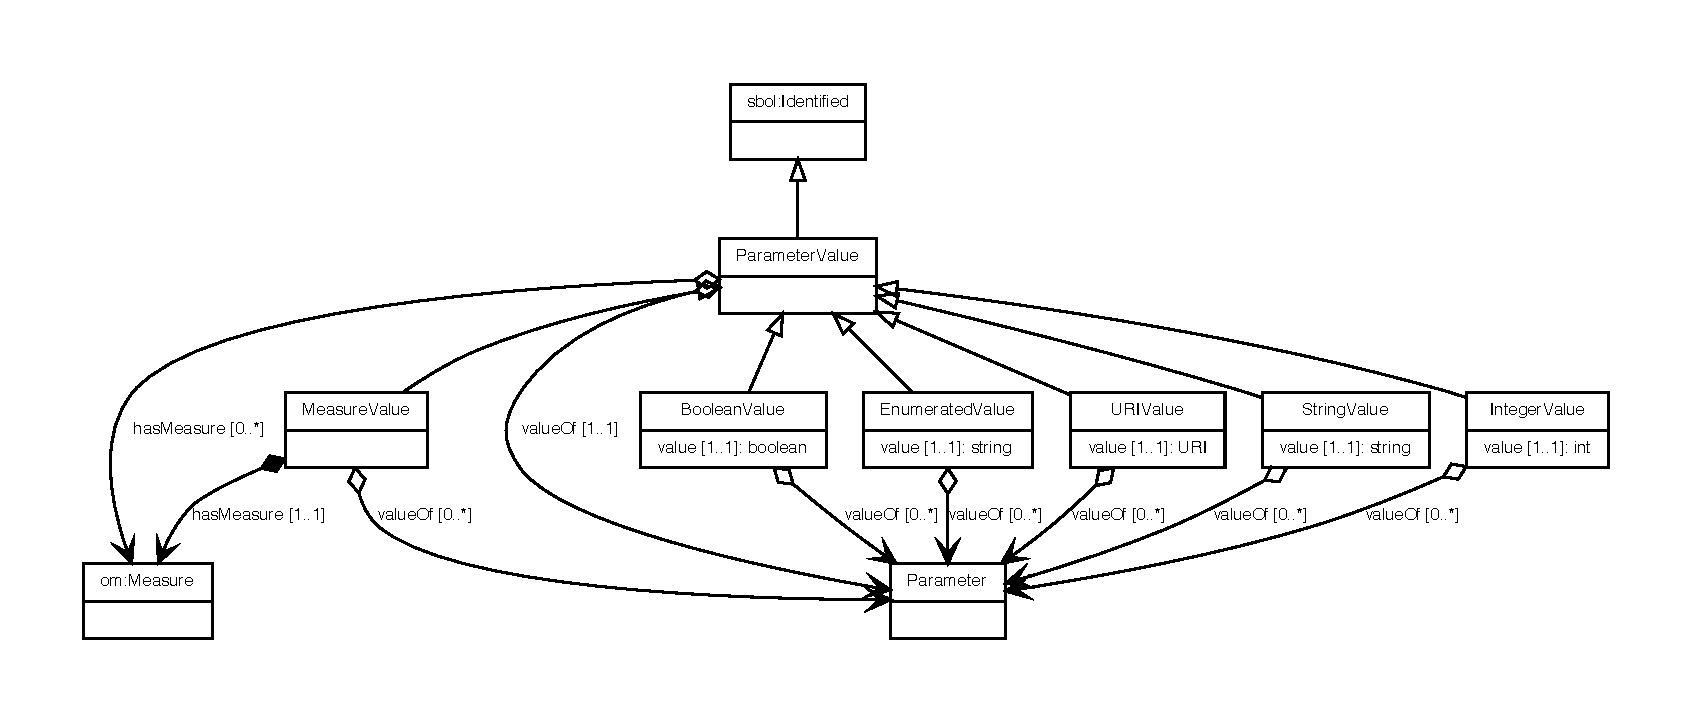
\includegraphics[scale=0.6]{figures/ParameterValue_definition_and_abstraction}
\caption[]{Diagram of the \opil{ParameterValue} abstract class and its associated properties and subclasses}
\label{uml:ParameterValue}
\end{center}
\end{figure}

\begin{itemize}
\item \label{sec:valueOf}
The \opil{valueOf} property is REQUIRED and MUST contain a single \opil{URI} that refers to the \opil{Parameter} describing the parameter being set.
The \opil{Parameter} MUST be of a corresponding class, e.g., a \opil{BooleanValue} must match a \opil{BooleanParameter}.
\end{itemize}


\subsubsection{BooleanValue}
\label{sec:BooleanValue}

\begin{itemize}
\item \label{sec:BP:value}
The \opilmult{BP:value}{value} property is REQUIRED and MUST contain a single \opil{boolean}.
\end{itemize}

\subsubsection{EnumeratedValue}
\label{sec:EnumeratedValue}

\begin{itemize}
\item \label{sec:EV:value}
The \opilmult{EV:value}{value} property is REQUIRED and MUST contain a single \opil{string} whose value is equal to one of the \opil{allowedValue} properties of the \opil{Parameter} referred to by the \opil{valueOf} property.
\end{itemize}


\subsubsection{IntegerValue}
\label{sec:IntegerValue}

\begin{itemize}
\item \label{sec:IV:value}
The \opilmult{IV:value}{value} property is REQUIRED and MUST contain a single \opil{integer}.
The value must be greater than or equal to that of the \opil{minValue} property (if set) of the \opil{Parameter} referred to by the \opil{valueOf} property, and less than or equal to the \opil{maxValue} property (if set).
\end{itemize}

\subsubsection{MeasureValue}
\label{sec:MeasureValue}

\begin{itemize}
\item \label{sec:hasValue}
The \opil{hasValue} property is REQUIRED and MUST contain a single \opil{URI} referring to a \om{Measure} object containing the value for the parameter.
The value of the linked \om{Measure} must be greater than or equal to that of the \opil{minMeasure} property (if set) of the \opil{Parameter} referred to by the \opil{valueOf} property, and less than or equal to the \opil{maxMeasure} property (if set).
\end{itemize}


\subsubsection{StringValue}
\label{sec:StringValue}

\begin{itemize}
\item \label{sec:SV:value}
The \opilmult{SV:value}{value} property is REQUIRED and MUST contain a single \opil{string}.
\end{itemize}


\subsubsection{URIValue}
\label{sec:URIValue}

\begin{itemize}
\item \label{sec:UV:value}
The \opilmult{UV:value}{value} property is REQUIRED and MUST contain a single \opil{URI}.
\end{itemize}










